\begin{filecontents}{\jobname.bib}
    %[1] (\cite{peteghem2010})
    @article{peteghem2010,
        title = {A genetic algorithm for the preemptive and non-preemptive multi-mode resource-constrained project scheduling problem},
        journal = {European Journal of Operational Research},
        volume = {201},
        number = {2},
        pages = {409-418},
        year = {2010},
        issn = {0377-2217},
        doi = {https://doi.org/10.1016/j.ejor.2009.03.034},
        url = {https://www.sciencedirect.com/science/article/pii/S037722170900191X},
        author = {Vincent Van Peteghem and Mario Vanhoucke}
    }
    %[2] (\cite{golmohammadi2015})
    @article{golmohammadi2015,
        title = {A study of scheduling under the theory of constraints},
        journal = {International Journal of Production Economics},
        volume = {165},
        pages = {38-50},
        year = {2015},
        issn = {0925-5273},
        doi = {https://doi.org/10.1016/j.ijpe.2015.03.015},
        url = {https://www.sciencedirect.com/science/article/pii/S0925527315000833},
        author = {Davood Golmohammadi}
    }
    %[3] (\cite{bofill2022})
    @article{bofill2022,
        title = {Constraint Solving Approaches to the Business-to-Business Meeting Scheduling Problem},
        journal = {Journal of Artificial Intelligence Research },
        volume = {74},
        pages = {263-301},
        year = {2022},
        doi = {https://doi.org/10.1613/jair.1.12670},
        url = {https://dl.acm.org/doi/pdf/10.1613/jair.1.12670},
        author = {Bofill,M. and Coll,C. and Garcia,M. and Giraldez-Cru,J. and Pesant,G. and Suy,J. and Villaret,M.}
    }
    %[4] (\cite{enembreck2012})
    @article{enembreck2012,
        title = {Distributed constraint optimization with MULBS: A case study on collaborative meeting scheduling},
        journal = {Journal of Network and Computer Applications},
        volume = {35},
        number = {1},
        pages = {164-175},
        year = {2012},
        note = {Collaborative Computing and Applications},
        issn = {1084-8045},
        doi = {https://doi.org/10.1016/j.jnca.2011.02.016},
        url = {https://www.sciencedirect.com/science/article/pii/S1084804511000543},
        author = {Fabrício Enembreck and Jean-Paul {André Barthès}}
    }
    %[5] (\cite{abuwarda2016})
    @article{abuwarda2016,
        title = {Work-Package Planning and Schedule Optimization for Projects with Evolving Constraints},
        journal = {Journal of Computing in Civil Engineering},
        volume = {30},
        number = {6},
        pages = {04016022},
        year = {2016},
        doi = {10.1061/(ASCE)CP.1943-5487.0000587},
        URL = {https://ascelibrary.org/doi/abs/10.1061/\%28ASCE\%29CP.1943-5487.0000587},
        author = {Zinab Abuwarda and Tarek Hegazy}
    }

    %[6] (\cite{marijn2011})
    @InProceedings{marijn2011,
        author = {Heule, Marijn J. H. and Kullmann, Oliver and Wieringa, Siert and Biere, Armin},
        editor = {Eder, Kerstin and Louren{\c{c}}o, Jo{\~a}o and Shehory, Onn},
        title = {Cube and Conquer: Guiding CDCL SAT Solvers by Lookaheads},
        booktitle = {Hardware and Software: Verification and Testing},
        year = {2012},
        publisher = {Springer Berlin Heidelberg},
        address = {Berlin, Heidelberg},
        pages = {50-65},
        volume = {7261},
        isbn = {978-3-642-34187-8},
        doi = {10.1007/978-3-642-34188-5_8}
    }
    %[7] (\cite{florian2009})
    @article{florian2009,
        author = {Berger, Florian and Klein, Rolf and Nussbaum, Doron and Sack, J\"{o}rg-R\"{u}diger and Yi, Jiehua},
        title = {A meeting scheduling problem respecting time and space},
        year = {2009},
        issue_date = {December  2009},
        publisher = {Kluwer Academic Publishers},
        address = {USA},
        volume = {13},
        number = {4},
        issn = {1384-6175},
        url = {https://doi.org/10.1007/s10707-008-0053-4},
        doi = {10.1007/s10707-008-0053-4},
        journal = {Geoinformatica},
        pages = {453-481}
    }
    %[8] (\cite{takuotsuruta})
    @article{takuotsuruta,
        author = {Takuo Tsuruta and Toramatsu Shintani},
        title = {Scheduling Meetings using Distributed Valued Constraint Satisfaction Algorithm}
    }
    %[9] (\cite{vincent2010})
    @article{vincent2010,
        author = {Peteghem, Vincent and Vanhoucke, Mario},
        year = {2010},
        month = {03},
        pages = {409-418},
        title = {A genetic algorithm for the preemptive and non-preemptive multi-mode resource-constrained project scheduling problem},
        volume = {201},
        journal = {European Journal of Operational Research},
        doi = {10.1016/j.ejor.2009.03.034}
    }
    %[10] (\cite{jiongzhi2024})
    @misc{jiongzhi2024,
        title={Rethinking the Soft Conflict Pseudo Boolean Constraint on MaxSAT Local Search Solvers}, 
        author={Jiongzhi Zheng and Zhuo Chen and Chu-Min Li and Kun He},
        year={2024},
        eprint={2401.10589},
        archivePrefix={arXiv},
        primaryClass={cs.AI},
        url={https://arxiv.org/abs/2401.10589}
    }
    %[10] (\cite{andrei2022})
    @article{andrei2022,
        title = {An overview of machine learning techniques in constraint solving},
        author = {Andrei Popescu and {Polat Erdeniz}, Seda and Alexander Felfernig and Mathias Uta and M{\"u}sl{\"u}m Atas and Le, {Viet Man} and Klaus Pilsl and Martin Enzelsberger and Trang Tran},
        year = {2022},
        doi = {10.1007/s10844-021-00666-5},
        volume = {58},
        pages = {91-118},
        journal = {Journal of Intelligent Information Systems},
        issn = {0925-9902},
        publisher = {Springer International Publishing AG},
        number = {1}
    }

    
\end{filecontents}
\documentclass[a4paper, 12pt]{article}
\usepackage[left=1in,right=1in,top=1in,bottom=1in]{geometry}
\usepackage{setspace}
\usepackage{titlesec}
\usepackage{graphicx}
\usepackage[section]{placeins}
\usepackage[bookmarks]{hyperref}
\usepackage[super]{nth}
\usepackage{subfig}
\usepackage{makeidx}
\usepackage{hyperref}
\usepackage{acronym}
\usepackage{array} 
\usepackage{mathrsfs}
\usepackage{amsmath}
\usepackage{amssymb}
\usepackage{multirow}
\usepackage{float}
\usepackage[backend=biber,style=authoryear,autocite=inline, maxbibnames=9 ]{biblatex}
\DeclareNameAlias{sortname}{last-first}
\addbibresource{\jobname.bib}
\graphicspath{ {images/} }
\newcolumntype{C}{>{$\displaystyle}l<{$}}

\makeindex

\begin{document}
    % 01 - Title page
    \newpage
    \pagenumbering{none}
    \begin{figure}
        \centering
        \vspace*{0cm}
\includegraphics[width=0.35\textwidth]{uoc_logo.jpg}
    \end{figure}
    \begin{center}
        \begin{LARGE}  
            \textbf{Privacy-Preserved Meeting Organization}
        \end{LARGE}  
        \break\break
        By\\
        \textbf{M.M.A.S.T. Akmeemana - Index No: 20020015\\ A.I. Vidanage - Index No: 20021089\\ K.P.G.K. Jayathilake - Index No: 20020521}
        \break\break
        \textbf{Supervisor: Dr. C.I. Kappetiyagama\\ Co-supervisor: Mr. Tharindu Wijethilaka}
        \break\break
        \begin{large}  
            IS 4101 – Final Year Project in Informatioon Systems
            \break\break
            Degree of Bachelor of Science Honours in\\ Information Systems
            \break\break
        \end{large}
        
        \begin{figure}[h]
            \centering
            
\includegraphics[width=0.3\textwidth]{ucsc_logo.png}
        \end{figure}
        \begin{large}  
            University of Colombo School of Computing\\
            35, Reid Avenue, Colombo 07,\\
            Sri Lanka\\
            April 2024
        \end{large}
    \end{center}

    % 02 - Table of Contents page
    \newpage
    \addcontentsline{toc}{section}{Table of Contents}
    \section*{\begin{LARGE} Table of Contents \end{LARGE} }
    \pdfbookmark{\contentsname}{toc}
    \tableofcontents

    \begin{spacing}{1.0}
    % 03 - Project profile
    \newpage
    \pagenumbering{arabic}
    \section{Project profile} 
    \subsection{Introduction}
    \indent \par A meeting is a synchronous communication, based on one or more documents, occurring at one or more locations. In today's interconnected world, meetings are held across various contexts and serve a multitude of purposes, from business discussions to academic collaborations. The organization of these meetings is increasingly supported by a range of platforms offered by different vendors, each designed to streamline the scheduling process and enhance user experience. Substantial research has focused on improving the quality and efficiency of meeting organization, addressing challenges such as preventing the overlap of participants in concurrent meetings or avoiding scheduling multiple meetings at the same location simultaneously. But, organizing meetings preserving privacy of meeting data remains an unexplored area. Current research has not adequately addressed the constraints necessary to safeguard meeting privacy, during the meeting scheduling process.
    
    \subsection{Motivation}
    \indent \par It is observed that the privacy of meetings is violated when they are organized in an ad-hoc manner. Because, when there are various topics to discuss, it is difficult to decide on participants relevant to each topic, without the help of a formal constraint resolution process. Privacy violation mainly takes place in the following manners.
    \begin{itemize}
        \item Adding unauthorized participants to meetings, such that they get access to confidential data restricted from them.
        \item Selecting privacy-violating meeting modes, in which meeting content can leak to unauthorized people.
    \end{itemize}

    \subsection{Scope}
    \begin{itemize}
        \item During identification of constraints related to the privacy of meetings, we have identified the following factors as constraints affecting the privacy of meetings.
        \begin{itemize}
            \item Meeting content
            \item Participants
            \item Meeting mode
        \end{itemize}
        \item Resolving identified constraints in a viable manner, producing an effective solution for supporting privacy-preserved meeting organization.
        \item Evaluating the solution to ensure the validity of the solution.
    \end{itemize}

    \newpage
    \subsection{Basic definitions}

    \subsubsection{Notations}
    \noindent
    Following finite sets are defined:
    \begin{itemize}
        \item $\mathcal{D}$: The set of all documents.
        \item $\mathcal{R}$: The set of all roles.
        \item $\mathcal{I}$: The set of all individuals
        \item $\mathcal{L}$: The set of all locations.
        \item $\mathcal{T}$: The set of all time slots.
    \end{itemize}

    \noindent
    Following functions are also defined:
        \[ access: \mathcal{D} \mapsto 2^\mathcal{R} \text{(} 2^\mathcal{R} \text{= power set of } \mathcal{R} \text{)} \] 
        \[ access(d) = \{ r \in \mathcal{R} \mid r \text{ has access to } d \} \] 
        \[ transform: \mathcal{I} \times \mathcal{L} \times \mathcal{T} \mapsto \mathcal{R} \] 
        \[ transform(i, l, t) = r : r \text{ is role of } i \text{ at location } l \text{ at time slot } t \] 
        \[ location: \mathcal{I} \times \mathcal{T} \mapsto \mathcal{L} \] 
        \[ location(i, t)  = l : i \text{ is at } l \text{ at } t \]

    \noindent
    A meeting M is a 4-tupple,
        \[ M = < D, I, L, t > \]
    such that,
        \[ D \subseteq \mathcal{D} \]
        \[ L \subseteq \mathcal{L} \]
        \[ I \subseteq \mathcal{I} \]
        \[ t \in \mathcal{T} \]

    \subsubsection{Access Control List}
    \noindent
    We define following 2 relationships.
    \[ d = \{ d \in \mathcal{D} \mid \text{d is a document} \} \]
    \[ i = \{ i \in \mathcal{I} \mid i \text{ is an individual } \} \]
    \[ g = \{ g \subseteq \mathcal{I} \mid g \text{ is a subset of one or more individuals in } \mathcal{I} \} \] \\ 
    
    \noindent
    Above relationships mean that $d$ is an element of set $\mathcal{D}$, and $i$ is an element of set $\mathcal{I}$. Further, $g$ is a group of one or more individuals ($i$), where $i \in \mathcal{I}$, such that $g \ne \emptyset$.\\ 

    \noindent
    Consider that following finite set is also defined:
    \begin{itemize}
        \item $\mathcal{G}$: Set of all possible not-null subsets of $\mathcal{I}$
    \end{itemize}
    Based on above all sets, we define following relationship.
    \[ access(d) = \{ g \in \mathcal{G} \mid g \text{ has access to } d \} \] \\ 
    \noindent
    Above relationship means that $g$ is an element of set $\mathcal{G}$, and that $access(d)$ is the set of groups ($g$) having access permission to document $d$.\\

    \subsubsection{Privacy-preserved meeting}
    \noindent
    \textbf{We assume that every meeting has an agenda document associated with it, to define the set of groups($g$) required to attend the meeting}\\
    \noindent
    A privacy-preserved meeting is a meeting in which individual $i$ representing role $r$ has no access to the meeting, when $r \in g$ and $g \notin access(agenda)$.

    \subsection{Aims}
    \begin{itemize}
        \item Resolving constraints associated with privacy-preserved meeting scheduling.
        \item Deciding the possibility of a privacy-preserved meeting to ensure the privacy of meeting content discussed, concerning the selected meeting participants.
        \item Selecting a privacy-preserving meeting mode, for conducting the particular meeting.
        \item Evaluating the solution in an acceptable, credible approach for ensuring its validity.
    \end{itemize}

    \subsection{Objectives}
    \begin{itemize}
        \item To map the identified constraints to a well-known constraint optimization problem.
        \item To determine whether a privacy-preserved meeting is possible depending on Access Control Lists (ACL) of documents associated with the meeting, based on the assumption that every meeting has at least one document associated with it (Meeting agenda document).
        \item To select a privacy-preserving meeting mode, based on availability and locations of selected meeting participants. 
        \item To evaluate the solution by defining an invariant set of rules, using a standard proof assistant (Ex: Coq, Isabelle, Lean)
    \end{itemize}




    % 04 - Literature survey and identified research gap
    \section{Literature survey and identified research gap}
    \subsection{Introduction to literature survey}
    \indent \indent Meeting scheduling becomes increasingly complex when incorporating privacy controls to restrict meeting access to authorized participants only. While many scheduling models address efficiency and availability, fewer approaches ensure access is controlled to prevent unauthorized participants from joining. This type of access-controlled privacy preservation is critical in sensitive or confidential meeting environments, such as corporate or client meetings, where unauthorized access could lead to security breaches. Despite notable advances, the field lacks a comprehensive, privacy-preserved scheduling model that fully addresses these needs. This literature review critically examines existing approaches, compares their methodologies and limitations, and identifies the gap in privacy-preserved meeting scheduling.
    
    \subsection{Literature survey}
    \subsubsection{Meeting Scheduling Challenges}
    \indent \indent Meeting scheduling that integrates access control requires decentralized management of permissions, which can be achieved through distributed models like Distributed Valued Constraint Satisfaction Problem (DVCSP) and Distributed Constraint Optimization Problem (DCOP). In these models, agents independently manage access for each participant, minimizing data sharing and reducing the risk of unauthorized access ( \cite{takuotsuruta} ;  \cite{enembreck2012}). 
    \par DVCSP and DCOP offer semi-optimal solutions with limited data exchange between agents, making them suitable for environments where meeting access needs to be restricted. However, while DVCSP allows for flexible constraint relaxation, it may fall short in settings where strict participant authorization is necessary. In contrast, the MULBS algorithm within DCOP provides a more secure option by focusing on minimal communication, reducing the risk of unauthorized access through limited information exposure.
    \par DVCSP’s main advantage is its flexibility, allowing agents to relax lower-priority constraints to achieve a balance between ideal scheduling and participant privacy. In contrast, DCOP uses independent agents to manage individual schedules with minimal data sharing, achieving semi-optimal solutions with lower computational costs. MULBS, a specific DCOP algorithm, emphasizes minimal communication requirements and privacy preservation, making it highly suitable for privacy-sensitive environments. Another distinct approach comes from GeoInformatica, which frames the scheduling problem within computational geometry, focusing on optimizing both time and spatial constraints through algorithms with O(n log n) complexity (\cite{florian2009}). 
    \par While DVCSP and DCOP both excel in preserving privacy through decentralized scheduling, they differ significantly in their computational approaches and the quality of solutions. DVCSP’s semi-optimal solutions are sufficient for low-density environments but may be inadequate in high-density scheduling contexts where optimization is critical. DCOP, particularly the MULBS algorithm, achieves greater computational efficiency by minimizing communication, yet it also sacrifices some scheduling accuracy due to its semi-optimal focus. GeoInformatica’s computational geometry-based model achieves excellent efficiency for time-space scheduling but does not address privacy directly, making it limited in privacy-sensitive scheduling environments.
    \subsubsection{Constraint-Based Optimization Techniques}
    \indent \indent Constraint-based optimization techniques like Constraint Programming (CP), Mixed-Integer Programming (MIP), and Maximum Satisfiability (MaxSAT) have been applied to scheduling, focusing on managing structured constraints around availability, priority, and location. CP allows for precise encoding of scheduling constraints, yet it lacks scalability in larger, more dynamic settings (\cite{bofill2022}). MIP, with its ability to rapidly identify infeasible solutions, is effective for structured scheduling tasks with rigid constraints but is too inflexible for applications with dynamic privacy needs (\cite{peteghem2010}). 
    \par Recent advances in MaxSAT, such as the Soft Conflict Pseudo Boolean (SPB) constraints, have introduced adaptive clause weighting strategies to improve local search efficiency in scheduling contexts. The SPB-MaxSAT algorithm, specifically, provides a high-performing solution for complex scheduling problems by adjusting clause weights to satisfy “soft” constraints, which are more flexible and adaptable (\cite{jiongzhi2024}). 
    \par CP and MIP serve well in traditional scheduling scenarios, but both fall short in contexts requiring real-time adaptability and privacy prioritization. While CP offers flexibility with strict constraints, its lack of scalability makes it unsuitable for larger, privacy-sensitive scheduling environments. MIP provides robust solutions for structured schedules but lacks the adaptability needed to handle frequent privacy-related adjustments. In comparison, MaxSAT—particularly the SPB-MaxSAT algorithm—introduces soft constraints that enable adaptability, positioning it as a more flexible alternative to CP and MIP. However, despite these improvements, MaxSAT lacks explicit privacy-focused mechanisms, meaning it primarily supports flexibility rather than privacy preservation.
    \par Overall, constraint-based techniques each contribute unique strengths to the scheduling field. CP’s precise encoding, MIP’s efficiency in identifying infeasible constraints, and MaxSAT’s adaptive clause weighting all provide valuable solutions to specific scheduling problems. Yet, the lack of real-time adaptability and privacy-preserving mechanisms across these methods underscores their limitations in handling complex, privacy-focused meeting scheduling scenarios. MaxSAT’s introduction of soft constraints offers the most promise for dynamic scheduling, but further integration with privacy-preservation techniques is essential to address privacy-sensitive needs fully.
    \subsubsection{Genetic Algorithms and Adaptive Scheduling}
    \indent \indent Genetic algorithms (GAs) introduce adaptability through iterative optimization, allowing for schedules to evolve based on changing constraints or resource availability. Applied extensively in resource-constrained scheduling, GAs use a bi-population model that supports continuous adjustments, which is advantageous in settings where participant availability and privacy needs fluctuate frequently (\cite{peteghem2010}). 
    \par GAs are more adaptable than constraint-based methods like CP and MIP, due to their iterative nature and ability to explore multiple solutions. This adaptability makes GAs suitable for environments with dynamic constraints, where immediate schedule adjustments are required. However, GAs’ computational intensity poses a challenge for real-time applications, particularly in privacy-sensitive contexts where participant selection may require immediate recalibration based on privacy needs. Compared to MaxSAT’s adaptive clause weighting, GAs offer greater flexibility but are less efficient computationally, requiring careful tuning of parameters to achieve optimal performance.
    \par The bi-population structure of GAs provides an advantage in dynamic environments, offering an adaptable alternative to more rigid constraint-based models. However, GAs are hindered by computational demands, which can limit their real-time responsiveness in privacy-sensitive scheduling. This indicates a need for hybrid approaches that incorporate GA adaptability with computational efficiency to better serve privacy-preserved meeting scheduling needs.
    \subsubsection{Theory of Constraints (TOC) and Bottleneck Management}
    \indent \indent The Theory of Constraints (TOC) focuses on identifying and alleviating bottlenecks within scheduling systems, improving throughput in resource-constrained environments. TOC has proven valuable in production-oriented scheduling, where specific bottlenecks often restrict scheduling efficiency and resource allocation (\cite{golmohammadi2015}). 
    \par While TOC is effective in managing resources and prioritizing critical constraints, it does not incorporate privacy considerations or adaptability for dynamic participant needs. In comparison, models like DVCSP and DCOP offer more delicate scheduling management by focusing on privacy through decentralized data management. While TOC targets throughput and bottleneck alleviation, its limited adaptability and lack of privacy mechanisms restrict its usefulness in privacy-sensitive scheduling environments.
    \par TOC’s bottleneck prioritization method is beneficial for environments where resource constraints drive scheduling but falls short in privacy-sensitive contexts. The rigid focus on throughput limits TOC’s applicability to meeting scheduling, which often requires flexible participant selection based on confidentiality needs. TOC’s strength in optimizing resource allocation could be enhanced with additional privacy and adaptability mechanisms to better address modern scheduling requirements.
    \subsubsection{Machine Learning and Hybrid Approaches in Constraint Solving}
    \indent \indent Machine learning (ML) enhances adaptive scheduling by using supervised learning to predict participant preferences and optimize scheduling algorithms based on past data. Hybrid models, such as Cube-and-Conquer, combine ML with traditional SAT solvers, improving scalability and efficiency in complex scheduling tasks (\cite{andrei2022} ; \cite{marijn2011}).
    \par ML’s ability to predict participant preferences makes it a valuable addition to adaptive scheduling, offering enhanced flexibility over CP, MIP, and TOC. In contrast to traditional models, ML enables real-time responsiveness to changing conditions, aligning well with the demands of privacy-preserved meeting scheduling. However, ML’s applications in privacy-sensitive contexts remain limited due to the absence of standardized privacy metrics and evaluation tools, which restricts its ability to fully manage confidentiality alongside scheduling.
    \par ML and hybrid models present significant opportunities for improving adaptability in scheduling through predictive capabilities. However, the lack of privacy-specific applications and standard metrics in ML means that its current role in privacy-preserved scheduling is limited. Developing standardized evaluation metrics and incorporating privacy mechanisms would enhance ML’s suitability for privacy-sensitive scheduling scenarios.
    \subsubsection{Privacy-Centric Distributed Models for Scheduling}
    \indent \indent Privacy-preserving scheduling has advanced through distributed models such as DCOP and DVCSP, which decentralize data management to protect participant confidentiality. The MULBS algorithm exemplifies the DCOP approach by minimizing communication among agents, which helps maintain privacy (\cite{enembreck2012}). GeoInformatica’s computational geometry-based approach addresses scheduling efficiency by using LP-type problems and graph models, but it lacks privacy-preserving mechanisms (\cite{florian2009}). 
    \par DCOP and DVCSP models emphasize privacy through minimal data exchange, contrasting with centralized approaches that are more susceptible to data exposure. MULBS’s minimal communication requirements make it highly suitable for privacy-sensitive contexts, while GeoInformatica’s time-space optimization algorithms provide efficiency but lack explicit privacy management. Compared to other scheduling models, these distributed approaches offer a balanced solution for privacy-sensitive environments but achieve only semi-optimal results due to the trade-off with computational efficiency.
    \par Distributed models effectively protect privacy but sacrifice some optimization to achieve this. DCOP and DVCSP’s decentralized approach addresses privacy needs better than centralized methods but falls short of delivering fully optimized solutions. There remains a gap in achieving optimal scheduling without compromising privacy, highlighting the need for models that can balance privacy, efficiency, and scheduling quality.

    \subsection{Research gap and conclusion}
    \indent \indent Despite significant advancements, privacy-preserving meeting scheduling remains largely unaddressed. Constraint-based methods excel in managing structured constraints but lack real-time adaptability and privacy-preserving mechanisms. Adaptive scheduling techniques, such as GAs and TOC, offer flexibility but fall short of the privacy requirements essential for modern scheduling contexts. Privacy-centric distributed models partially address privacy needs but achieve only semi-optimal outcomes, highlighting a clear research gap.
    \par Future research must focus on developing hybrid scheduling models that integrate constraint-based optimization, machine learning, and distributed frameworks to create secure, responsive, and privacy-focused scheduling solutions. Addressing this gap would advance the field, providing compliant, adaptable scheduling frameworks tailored to modern privacy-sensitive environments.


    % 05 - Revised research question
    \section{Research question}
    \subsection{Hypothesis}
    \par \textbf{Meeting participant selection} is primarily dominated by the access control lists of the \textbf{documents} presented including meeting agenda, and the choice of \textbf{meeting mode} depends on the participants’ locations.
    \subsection{Research question statement}
    \par What is the algorithm to validate the above hypothesis ?
    
    % 06 - Research approach
    \section{Research approach}
    \begin{enumerate}
        \item Identify and define constraints associated with privacy-preserved meeting organization.
        \item Map the identified constraints to a well-known constraint optimization problem.
        \item Evaluate the finalized solution by defining an invariant set of rules, using a standard proof assistant (Ex: Coq, Isabelle, Lean).
    \end{enumerate}

    % 07 - Experiments and preliminary results
    \section{Experiments and preliminary results}
    \subsection{Experiments}
        \begin{itemize}
            \item We have started to define constraints associated with privacy-preserved meeting organization. The latest version of currently identified constraints and defined concepts is included in the following document. This content is to be further fine-tuned in the future, depending on our findings in this research. 
                \begin{itemize}
                    \item \url{https://github.com/Thejana-A/IS-4101-git/blob/master/latex/definitions_Sep_20/definition.pdf} 
                \end{itemize}
            \item We have developed a basic workflow in Python, including steps for,
                \begin{itemize}
                    \item Meeting participant validation, based on Access Control Lists of documents related to the meeting, including meeting agenda. 
                    \item The meeting time slot selection based on the availability of validated participants.
                    \item Meeting mode selection based on the locations of participants, during the eligible time slot.
                \end{itemize}
            \item This basic workflow was implemented using a set of functions present in Python language. Its latest version is available at the following link.
                \begin{itemize}
                    \item \url{https://github.com/Thejana-A/IS-4101-git/blob/master/python_code/intersection_nov04.py } 
                \end{itemize}
            \item For resolving privacy-preseved meeting constraints in more optimum manner, we need to map above mentioned 3 steps of workflow to eligible well-known constraint optimization algorithms. Because, it is not feasible to evaluate all possibilities in problem space for a solution developed from scratch, regarding our constraint resolving problem.
            \item Meeting constraint optimization research conducted by Bofill et al concluded that MaxSAT was the best algorithm for their research problem (\cite{bofill2022}). Therefore, we decided to analyze the MaxSAT algorithm to check whether it is eligible for our meeting constraint resolving problem as well.
            \item Currently, we are analyzing the following MaxSAT implementations simultaneously, to see whether they can satisfy our constraint resolving requirement regarding \textbf{meeting participant validation, based on Access Control Lists of documents related to the meeting}.
                \begin{itemize}
                    \item Pure MaxSAT algorithm: 
                        \begin{itemize}
                            \item \url{https://github.com/sukrutrao/MaxSAT-Solver}
                        \end{itemize}
                    \item Partial weighted MaxSAT algorithm: 
                        \begin{itemize}
                            \item \url{https://github.com/FlorentAvellaneda/EvalMaxSAT}
                        \end{itemize}
                    \item Both Pure and partial weighted algorithms:
                        \begin{itemize}
                            \item \url{https://github.com/pysathq/pysat/blob/master/solvers/glucose30.tar.gz}
                            \item \url{https://github.com/pysathq/pysat/blob/master/solvers/glucose421.tar.gz}
                        \end{itemize}
                \end{itemize}
            \item We have used inputs created by ourselves and exhaustive input sets available at the following link, for analyzing the above MaxSAT solvers, by observing the output delivered for various inputs.
                \begin{itemize}
                    \item \url{https://github.com/harshad-p/max-sat-solver/tree/master/input}
                \end{itemize}
        \end{itemize}
    
    \subsection{Current progress}
    \begin{itemize}
        \item For now, none of the above MaxSAT solvers were capable of providing promising support for resolving constraints related to \textbf{meeting participant validation}. We hope to analyze them further, before shifting to a different algorithm, to check whether any of these MaxSAT algorithms can be mapped to our constraint resolving requirement successfully.
    \end{itemize}

    % 08 - Finalized evaluation plan
    \section{Finalized evaluation plan}
    \indent \indent If a solution is developed from scratch for our constraint resolving problem, it is difficult to evaluate the finalized solution (proof of concept) experimentally, since there are extremely large number of possibilities for meetings in problem space.\\
    \par Accordingly, we are planning to formally map our constraint resolving problem to a well-known constraint optimization problem, which is already addressed. We hope to develop an invariant set of rules for ensuring validity of that mapping.
    In addition, those invariant rules will be proven by using a standard proof assistant (Ex: Coq, Isabelle, Lean), to reinforce the credibility.
    

    % 09 - Significance of the project with regards to research contribution to Information Systems and other areas such as benefits to society
    %\section{Research contribution to Information Systems and benefits to the society}

    % 10 - Project timeline and current progress
    %\section{Project timeline and current progress}
    %\subsection{Project timeline}
    %\begin{figure}[h!]
        %\centering
        %\vspace*{0cm}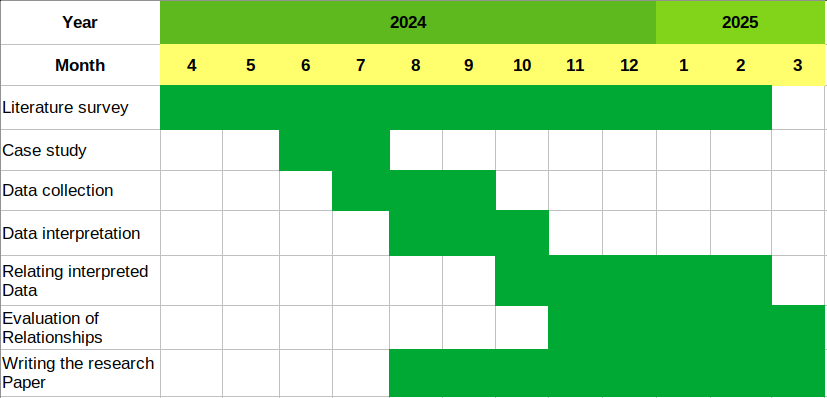
\includegraphics[width=0.65\textwidth]{timeline.png}
        %\caption{Planned project timeline}
    %\end{figure}

    \end{spacing}

    %List of References 
    \newpage
    \addcontentsline{toc}{section}{List of References }
    \section*{\begin{LARGE} List of References  \end{LARGE} }
    \printbibliography

\end{document}